\documentclass{article}
\usepackage{graphicx}
\usepackage{tabularx}
\usepackage{fancyhdr}
\usepackage{cite}
\usepackage{hyperref}
\usepackage{lipsum}
\usepackage{xcolor}
\usepackage{colortbl}

\pagestyle{fancy}
\setlength{\footskip}{60pt}
\vspace{-2cm}
\fancyfoot{\rule{0.5\linewidth}{1pt}}
\fancyfoot[L]{{
\includegraphics[scale=0.10]{logo.png}}}

\definecolor{lightgreen}{rgb}{0.56, 0.93, 0.56}

\begin{document}


\begin{center}

\includegraphics[scale=0.2]{logo.png}
\end{center}

\vspace{0.5cm}

\begin{center}

 Team's name: FamilyName1, FamilyName2, FamilyName3, FamilyName4 \\

\vspace{0.5cm}

{\Huge \textcolor{red}{Recovery and stress meter}} \\


\vspace{0.5cm}

{\Large \textbf{Requirement Specifications}} \\


\end{center}

\vspace{1cm}

\begin{center}

{\Large }



\begin{tabular}{l}
 First year hardware project \\
 School of ICT\\
 Metropolia University of Applied Sciences  \\
 \today \, (v1.1)
\end{tabular}
\end{center}

\newpage

\begin{abstract}
Write your abstract here.
\end{abstract}





\begin{table}[h]
\centering
\caption{Version history}
\label{tab:version_history}
\begin{tabular}{|c|p{5cm}|c|l|}
\hline
\textbf{Ver} & \textbf{Description} & \textbf{Date} & \textbf{Author(s)} \\
\hline
0.1 & First draft. Translated from Finnish template. & 23.9.2022 & SL \\
\hline
0.2 & Working principle added to the introduction. Description of the current situation added. & 24.11.2022 & SL \\
\hline
0.3 & Description of the target state added. & 25.11.2022 & SL \\
\hline
0.4 & Continuing description of the target state. & 28.11.2022 & SL \\
\hline
0.5 & Added heart rate detection and heart rate variability to Ch 3. Edited Ch 4. Added key features, use and users, and platforms of application. & 2.12.2022 & SL \\
\hline
0.6 & Added first draft of functional and non-functional requirements, users and use cases & 3.12.2022 & SL \\
\hline
0.7 & Updated non-functional requirements. Minor changes and proof reading. & 11.12.2022 & SL \\
\hline
0.8 & Some language corrections up to 3.3. May need further correcting. & 13.12.2022 & SH, SL \\
\hline
0.9 & Final reviews before release to workspaces & 19.12.2022 & SL \\
\hline
1.0 & Added Table 3. Components & 23.1.2023 & SL \\
\hline
1.1 & Some minor language corrections and updates & 25.1.2023 & S \\
\hline
\end{tabular}
\end{table}

\pagebreak

\tableofcontents

\newpage

\section{Introduction}
This document is part of a hardware project for the first year ICT engineering students
studying at Metropolia University of Applied Sciences. The aim of this document is to give
the requirement specifications for a new health technology device for measuring recovery
and stress index using optically detected heart rate and its variability.
The state of the autonomous nervous system (ANS) can be estimated from the heart rate
variation. Nowadays most of the wearable activity tracking devices and sports watches
detect the heart rate and its variability either electrically (e.g. detecting the electrocardiogram
or some parts of its signal) or optically (e.g. optical heart rate detector or oxygen saturation
detectors). [1]
Heart rate variability (HRV) is an accurate method to assess the autonomic nervous system
(ANS) function. HRV is widely used by health and wellbeing professionals to objectively
measure the physiological and mental stress and recovery. In addition, HRV is a commonly
used tool in the research of different cardiovascular and metabolic diseases and their risk
factors. [2]
The aim for the project is to build an objective and easy to use device for measuring HRV
and estimate the current stress or recovery status. The device is intended to be used in
home or office environments either by the end users themselves or together with health and
wellbeing professionals such as physiotherapists, nurses or medical doctors.
The device detects the heart rate and its variability using a photoplethysmography (PPG). It
measures optically blood volume changes in the microvascular bed of tissue. The change in
volume is detected by measuring the light emitted by the light emitting diodes (LEDs),
absorbed by the tissues and detected with photodiodes. The heart rate can be measured
from the peaks of the alternating signal presenting the volumetric blood changes in the
tissue. [3]

\pagebreak

\section{Concepts and definitions}
\begin{table}[h]
\label{tab:deliverable}
\resizebox{0.75\columnwidth}{!}{
\begin{tabular}{p{2cm} p{9cm}}
$\alpha$ & Slope of the linear interpolation of the spectrum in a log-log scale \\
ANS & Autonomous nervous system \\
BPM & Beat per minute \\
ECG & Electrocardiogram \\
IBI & Inter-beat-interval, measured from PPG signal, given in milliseconds (ms) \\
HF & High frequency \\
HR & Heart rate, typically given in units of beat per minute (BPM) \\
HRV & Heart rate variability, measures how much there is variability in the heart rate from  beat to beat over longer time period, can be characterized by several parameters  \\
LAN & Local area network \\
LED & Light emitting diode \\
LF & Low frequency \\
LF/HF & Ratio of LF/HF \\
NN  interval & Time difference between two peaks either in ECG or PPG signal, either PPI and RRI \\
NN50 count & Number  of pairs of adjacent NN intervals differing more than 50 ms \\
OLED & Organic light emitting diode \\
pNN50 & NN50 count divided by the total number of all NN intervals \\
PPI & peak-to-peak interval, time difference between two pulse peaks in photoplethysmography signal \\
PPG & Photoplethysmography, optically detected heart pulse typically detected from peripheral blood circulation, like from finger, wrist, toe, or ear lobe \\
PNS & Parasympathetic nervous system, part of autonomic nervous system \\
PTSD & Post-traumatic stress disorder \\
RMSSD & The square root of sum of squares of differences (ms) \\
RRI & RR-interval, time difference between two R-peaks in ECG signal \\
SD1 & Poincaré plot index \\
SD2 & Poincaré plot index \\
SDANN & Standard deviation of the average of NN intervals (ms) \\
SDNN & Standard deviation of all NN intervals (ms) \\
SI & Baevsky’s stress index \\
SDSD & Standard deviation of differences between adjacent NN intervals (ms) \\
SNS & Sympathetic nervous system, part of autonomic nervous system \\
ULF & Ultra-low frequency \\
USB & Universal serial port \\
WiFi & Wireless fidelity \\
VLF & Very flow frequency \\
\end{tabular}
}
\end{table}

\pagebreak

\section{Description of the current situation}
\subsection{Stress}
Stress is defined as “a physical, mental, or emotional factor that causes bodily or mental
tension” [4]. According to the American Institute of Stress [5] [6]:

\begin{itemize}
\item 77 \% of people experience stress that affects their physical health
\item 73 \% of people have stress that impacts their mental health
\item 48 \% of people have trouble sleeping because of stress
\item 33 \% of people report feeling extreme stres
\end{itemize}

[Figure]

Physiological or mental imbalance can induce stress. Our autonomic nervous system (ANS)
quickly responds with physiological changes through our sympathetic (SNS) and
parasympathetic (PNS) nervous systems. During the stress response our body’s endocrine
system releases hormones, and several changes in our physiological state occur. For
example, heart rate (HR) can even double or triple and causes changes to HRV. [8]

\subsection{Detecting heart rate}
The heart rate or pulse rate measures how often the heart beats and is given units of beats
per minute (BPM). Usually, the heart rate varies on the body’s physical need, but is also
affected by physical fitness, stress of psychological status, diet, drugs, hormones,
environment and diseases and illnesses. The normal resting adult heart rate is 60-100 BPM.
During sleep, a heart rate of 40-50 BPM is common and considered normal. [9]

4 (16)
Heart rate variability (HRV) is the variation of the time intervals between heartbeats and it is
measured in units of seconds, or more commonly, in milliseconds (ms). Other terms used
include RR interval (RRI) variability, where R corresponds to the peak of QRS-complex of
electrocardiography (ECG), and Peak-to-Peak interval, if the HRV is measured optically.
Figure 2 visualizes heart HRV with R-R interval changes. [10]

[Figure]

Heart rate variability can be detected with various methods. ECG is considered the golden
standard for HRV measurement [10]. Other methods are photoplethysmography (PPG),
which detects the heart rate variability optically, usually measured from fingers, wrists,
forehead or earlobes, blood pressure or ballistocardiography, which measures small
changes in body’s weight when the blood flows from the heart to the aorta.

[Figure]

Figure 4 shows an example of photoplethysmography signal recorded with wrist worn pulse
oximetry [12]. The device is shown on the left. The sensor is attached to the thumb. The
PPG signal is shown on the right. The inter-beat-interval (IBI) is calculated from the negative
peaks (the bottoms) of the PPG signal. It could be calculated also from the positive peaks
(the maximum) or from the rising edges of the signal.

[Figure]

\subsection{Heart rate variability}
At present there is no accepted standard for stress evaluation. However, several HRV
variables change in response to stress. Usually, stress induces low parasympathetic
nervous system activity, which is associated with variation of some HRV variables such as
high-frequency band and an increase in the low-frequency band. [8]
European Society of Cardiology together with the North American Society of Pacing and
Electrophysiology have defined and established the standards for the measurement,
physiological interpretation, and clinical use of HRV [13]. Most used selected time-domain
and frequency-domain measures of HRV are summarized in Table 1 and Table 2.

\subsection{Recovery and stress indexes}

\section{Description of the target state}
\subsection{The purpose}
\subsection{Application concept}
\subsection{Operating principle}
\subsection{Key features}
\subsection{Use and users}
\subsection{Applications}

\section{Functional requirements}

\section{Non-functional requirements}

\section{Use cases}
\subsection{User roles}
\subsection{Use cases and use case diagram}
\subsection{Detailed description of the use cases}

\label{sec:references}
%%%%%%%%%%%%%%%%%%%%%%%%%%%%%%%%%%%%%%%%%%%%%%%%%%%%%%%%%%%%%%%%%%%%%%%%%%%%%



\begin{figure*}[h]
  \centering
  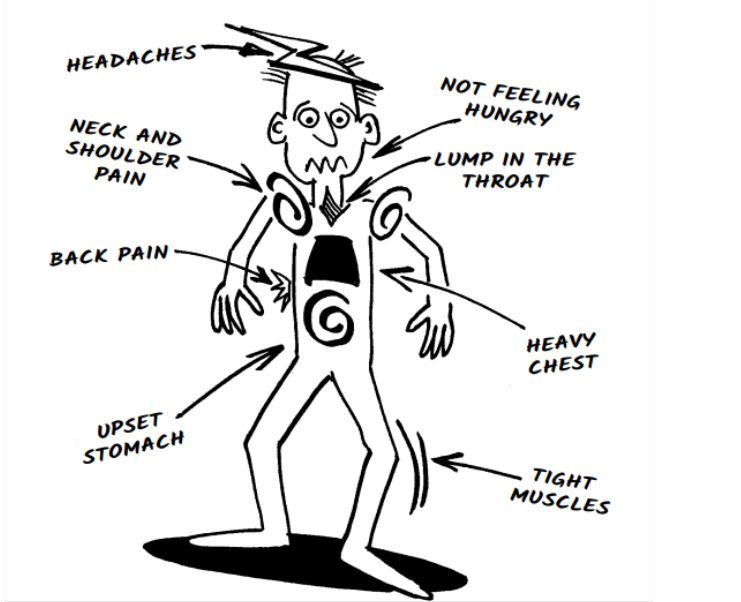
\includegraphics[width=0.7\textwidth]{sick.png}
  \caption{ Example of project's organisational chart (Source: Harrin, 2017).}
  \label{harrin}
\end{figure*}



\begin{figure*}[h]
  \centering
  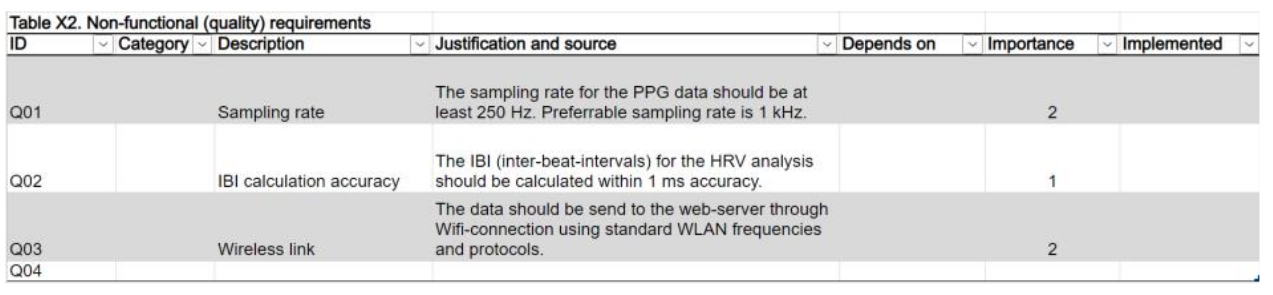
\includegraphics[width=0.7\textwidth]{screenshot2.png}
  \caption{ Example of project's organisational chart (Source: Harrin, 2017).}
  \label{harrin}
\end{figure*}

\begin{figure*}[h]
  \centering
  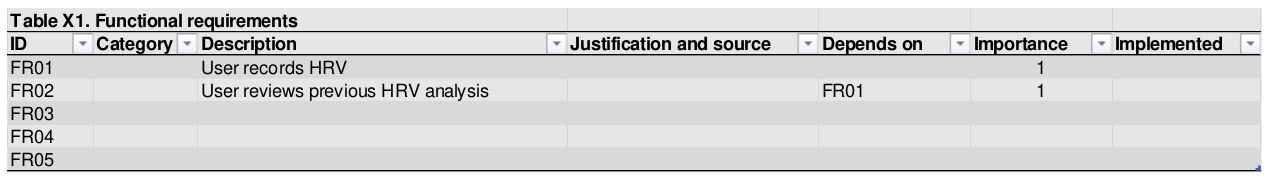
\includegraphics[width=0.7\textwidth]{screenshot.png}
  \caption{ Example of project's organisational chart (Source: Harrin, 2017).}
  \label{harrin}
\end{figure*}



\begin{figure*}[h]
  \centering
  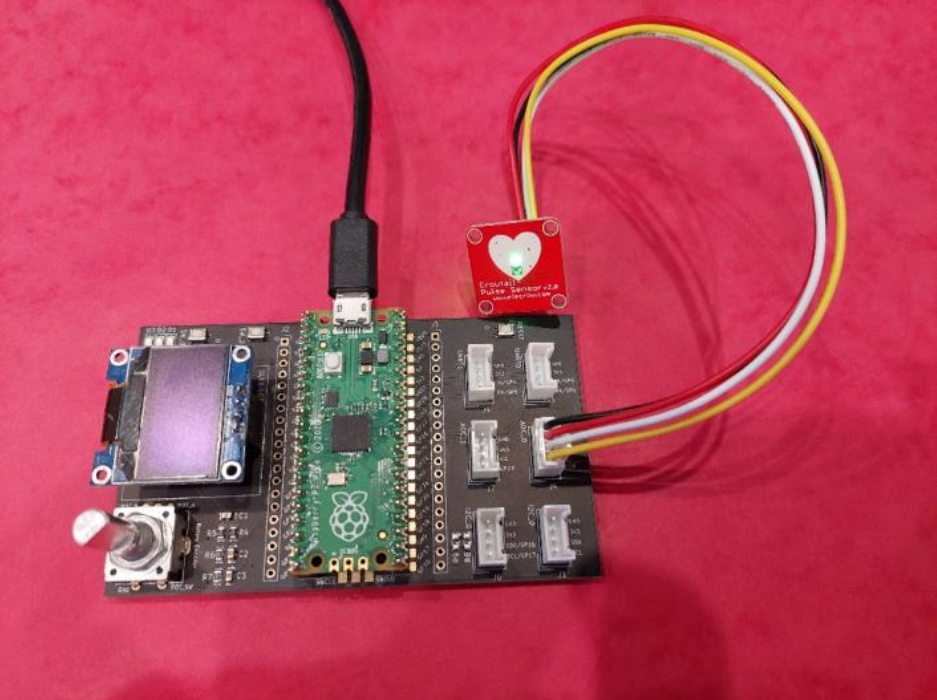
\includegraphics[width=0.7\textwidth]{raspi_heart.png}
  \caption{ Example of project's organisational chart (Source: Harrin, 2017).}
  \label{harrin}
\end{figure*}



\begin{figure*}[h]
  \centering
  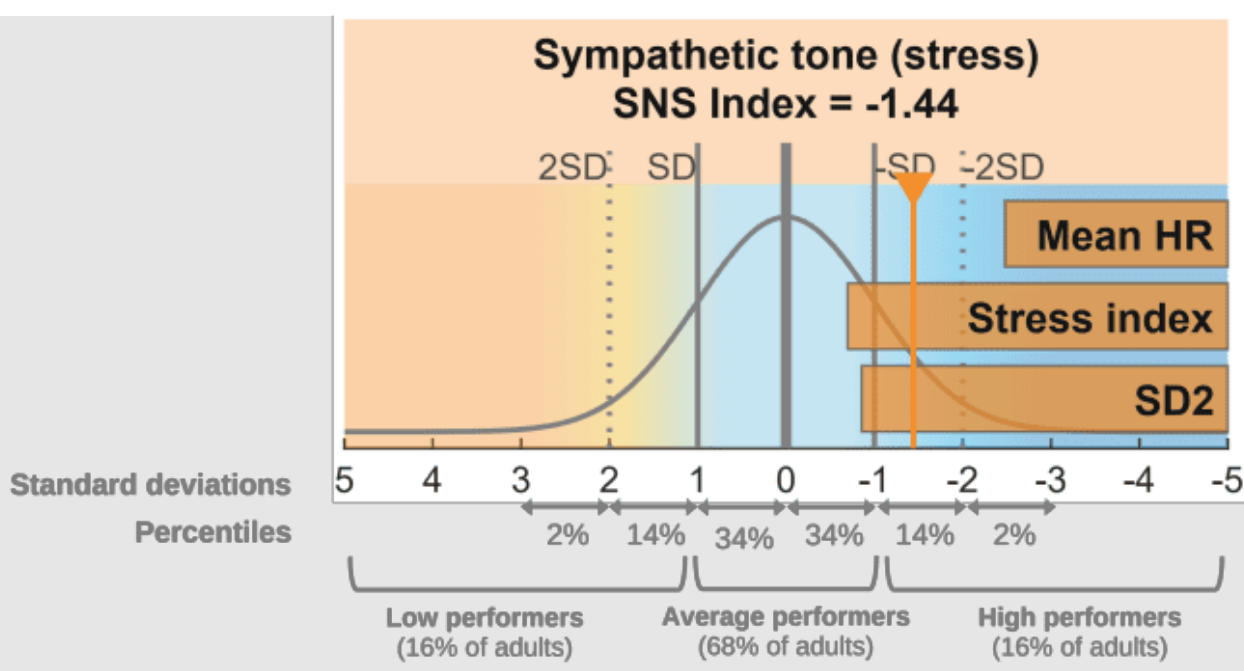
\includegraphics[width=0.7\textwidth]{sympathetic2.png}
  \caption{ Example of project's organisational chart (Source: Harrin, 2017).}
  \label{harrin}
\end{figure*}



\begin{figure*}[h]
  \centering
  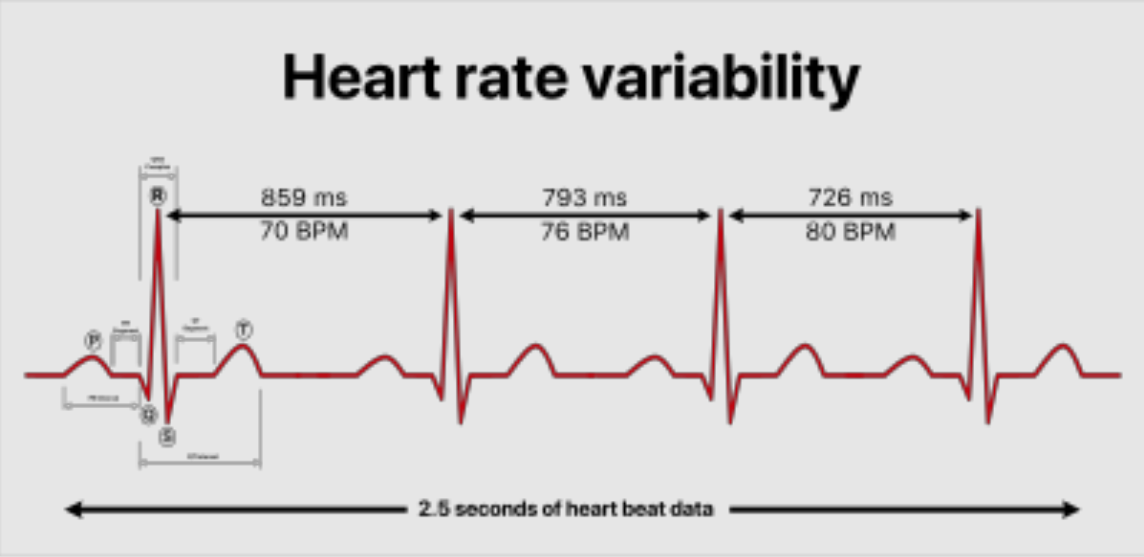
\includegraphics[width=0.7\textwidth]{heart_rate.png}
  \caption{ Example of project's organisational chart (Source: Harrin, 2017).}
  \label{harrin}
\end{figure*}



\begin{figure*}[h]
  \centering
  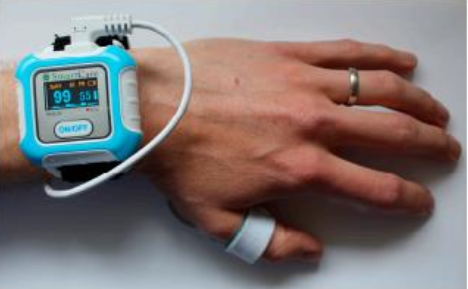
\includegraphics[width=0.7\textwidth]{hand.png}
  \caption{ Example of project's organisational chart (Source: Harrin, 2017).}
  \label{harrin}
\end{figure*}


\begin{figure*}[h]
  \centering
  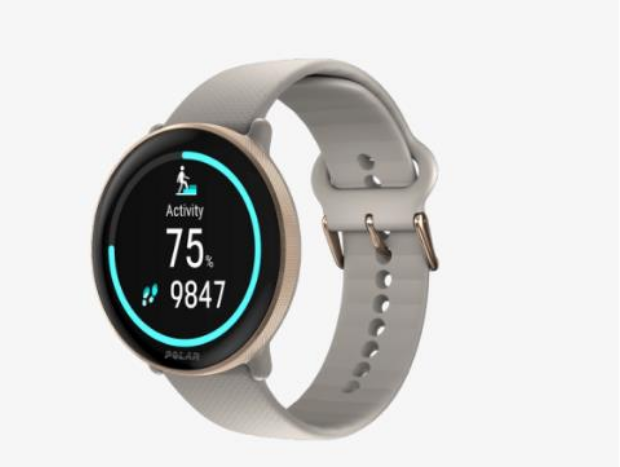
\includegraphics[width=0.7\textwidth]{watch1.png}
  \caption{ Example of project's organisational chart (Source: Harrin, 2017).}
  \label{harrin}
\end{figure*}


\begin{figure*}[h]
  \centering
  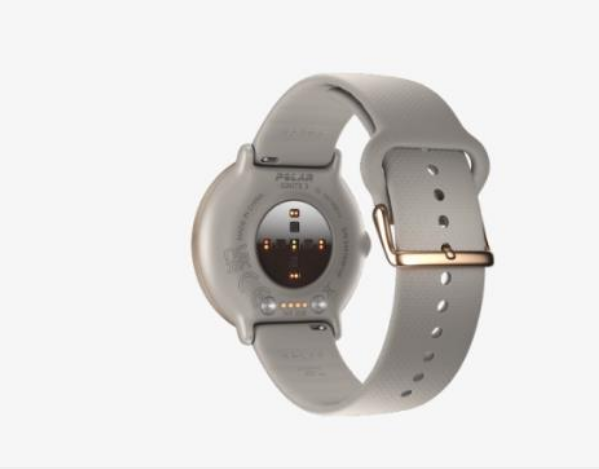
\includegraphics[width=0.7\textwidth]{watch2.png}
  \caption{ Example of project's organisational chart (Source: Harrin, 2017).}
  \label{harrin}
\end{figure*}
\begin{figure*}[h]
  \centering
  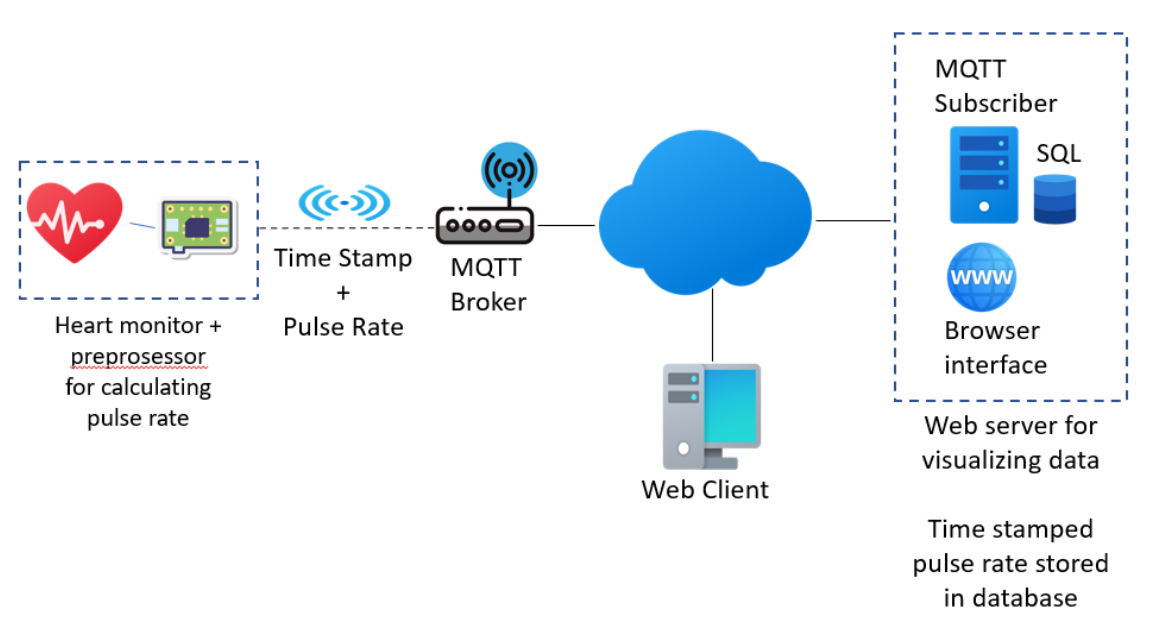
\includegraphics[width=0.7\textwidth]{web_server.png}
  \caption{ Example of project's organisational chart (Source: Harrin, 2017).}
  \label{harrin}
\end{figure*}

\begin{figure}[h]
\begin{minipage}{0.5\textwidth}
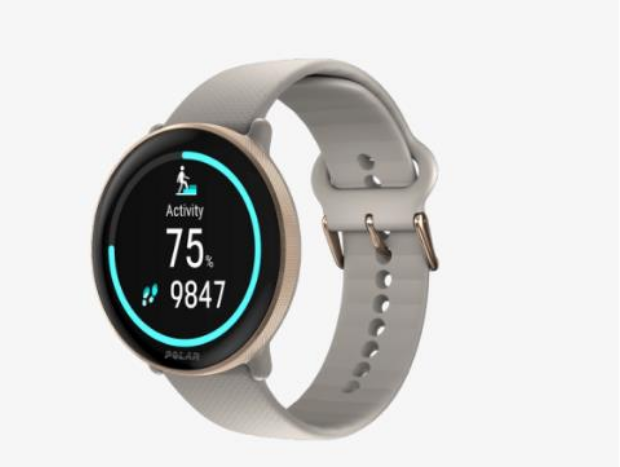
\includegraphics[width=\linewidth]{watch1.png}
\label{fig:sub1}
\end{minipage}
\begin{minipage}{0.5\textwidth}
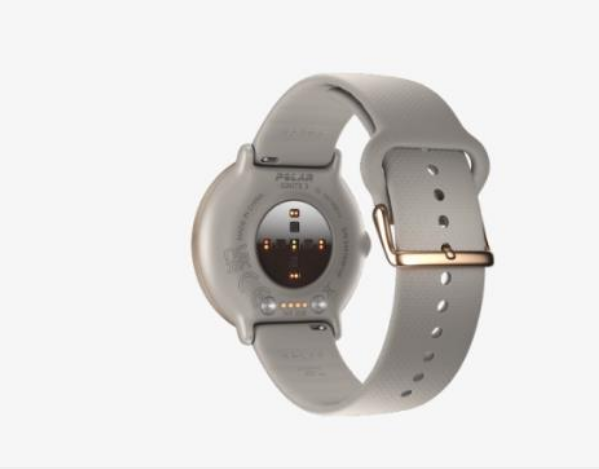
\includegraphics[width=\linewidth]{watch2.png}
\label{fig:sub2}
\end{minipage}
\caption{Caption for both figures}
\label{fig:test}
\end{figure}

\begin{table}[h]
\centering
\caption{Selected time-domain measures of HRV [13]}
\label{tab:HRV}
\begin{tabular}{llp{7cm}}
\hline
\textbf{Variable} & \textbf{Units} & \textbf{Description} \\ \hline
SDNN & ms & Standard deviation of all NN intervals \\ \hline
SDANN & ms & Standard deviation of the averages of NN intervals in all 5-minute segments of the entire recording \\ \hline
RMSSD & ms & The square root of the mean of the sum of the squares of differences between adjacent NN intervals \\ \hline
SDNN index & ms & Mean of the standard deviations of all NN intervals for all 5-minute segments of the entire recording \\ \hline
SDSD & ms & Standard deviation of differences between adjacent NN intervals \\ \hline
NN50 count & ms & Number of pairs of adjacent NN intervals differing by more than 50 ms in the entire recording \\ \hline
pNN50\% & - & NN50 count divided by the total number of all NN intervals \\ \hline
HRV triangular index & ms & Total number of all NN intervals divided by the height of the histogram of all NN intervals \\ \hline
TINN & ms & Baseline width of the minimum square difference triangular interpolation of the highest peak of the histogram of all NN intervals \\ \hline
Differential index & ms & Difference between the widths of the histogram of differences between adjacent NN intervals measured at selected heights \\ \hline
Logarithmic index & - & Coefficient $\phi$ of the negative exponential curve $k · e^{-\phi t}$, which is the best approximation of the histogram of absolute differences between adjacent NN intervals \\ \hline
\end{tabular}
\end{table}


\begin{table}[h]
\centering
\caption{Selected frequency-domain measures of HRV [13]}
\label{tab:HRV_freq}
\begin{tabular}{|l|l|l|}
\hline
\textbf{Variable} & \textbf{Units} & \textbf{Description} \\ \hline
\multicolumn{3}{|c|}{\textbf{Analysis of short-term recordings (5 min)}} \\ \hline
5min total power & ms$^2$ & The variance of NN intervals over the temporal segment \\ \hline
VLF & ms$^2$ & Power in VLF range (buffer 0.4 Hz) \\ \hline
LF & ms$^2$ & Power in LF range (0.04–0.15 Hz) \\ \hline
LF norm & n.u. & LF power in normalized units (LF/(total power-VLF)×100) \\ \hline
HF & ms$^2$ & Power in HF range (0.15–0.4 Hz) \\ \hline
HF norm & n.u. & HF power in normalized units (HF/(total power-VLF)×100) \\ \hline
LF/HF & - & Ratio LF/HF \\ \hline
\multicolumn{3}{|c|}{\textbf{Analysis of entire 24 hours}} \\ \hline
Total power & ms$^2$ & Variance of all NN intervals \\ \hline
ULF & ms$^2$ & Power in the ULF range (buffer 0.003 Hz) \\ \hline
VLF & ms$^2$ & Power in the VLF range (0.003–0.04 Hz) \\ \hline
LF & ms$^2$ & Power in the LF range (0.04–0.15 Hz) \\ \hline
HF & ms$^2$ & Power in the HF range (0.15–0.4 Hz) \\ \hline
$\alpha$ & ms$^2$ & Slope of the linear interpolation of the spectrum in a log-log scale \\ \hline
\end{tabular}
\end{table}

\begin{table}[h]
\centering
\caption{Component used in the proof-of-concept product.}
\label{tab:POC_components}
\begin{tabular}{|l|p{5cm}|}
\hline
\textbf{Component} & \textbf{Description} \\ \hline
Raspberry Pi & Dual-core ARM processor microcontroller having 246 kB SRAM and 2 MB on-board Flash. It also includes 2.4 GHz wireless LAN and 26 multifunction GPIO pins.\\ \hline
Crowtail Pulse Sensor v2.0 & Optical heart rate sensor with LED, photodiode, analog amplifier, and analog signal output. Operating voltage 3-5 V. \\ \hline
OLED Display & SSD1306 compatible 128x64 monochrome organic LED-display. Communicates with I2C or UART-protocol. \\ \hline
Protoboard & Passive protoboard specially designed for this project to help connect the other components to the Raspberry Pi. \\ \hline
Rotary knob & Digital rotary knob with push button. \\ \hline
\end{tabular}
\end{table}



\begin{table}[h]
\centering
\caption{Component used in the proof-of-concept product.}
\label{tab:POC_components}
\begin{tabular}{|l|p{5cm}|l|}
\hline
\textbf{Component} & \textbf{Description} & \textbf{More Info} \\ \hline
Raspberry Pi & Dual-core ARM processor microcontroller having 246 kB SRAM and 2 MB on-board Flash. It also includes 2.4 GHz wireless LAN and 26 multifunction GPIO pins. & Raspberry Pi website \\ \hline
Crowtail Pulse Sensor v2.0 & Optical heart rate sensor with LED, photodiode, analog amplifier, and analog signal output. Operating voltage 3-5 V. & Elecrow website \\ \hline
OLED Display & SSD1306 compatible 128x64 monochrome organic LED-display. Communicates with I2C or UART-protocol. & SSD1306 OLED Display datasheet \\ \hline
Protoboard & Passive protoboard specially designed for this project to help connect the other components to the Raspberry Pi. & N/A \\ \hline
Rotary knob & Digital rotary knob with push button. & N/A \\ \hline
\end{tabular}
\end{table}


\begin{table}
\begin{tabular}{|p{4cm}|p{7cm}|}
\hline
\textbf{Key Feature} & \textbf{Description} \\
\hline
HRV detection & PPG signal is detected using the optical pulse sensor and the heart rate variability is measured using the development board’s MCU. \\
\hline\
Display & The system has an OLED display capable of showing both text and graphics. \\
\hline\
Controls & The system has a rotary switch control knob with push button. The control knob can be used for controlling the operation of the system. \\
\hline
MCU & The system contains an MCU with Flash and RAM memory and several peripheral connections enabling to process the detected PPG signal and calculate the inter-peak-interval variations. \\
\hline
Wireless connection & The raw HRV data (PPI) can be further analysed using the system or sent wirelessly to a Cloud Server for further calculations. The system contains a wireless WiFi transmitter. \\
\hline
USB connection & The system contains a USB connection. The USB can be used to control, code, and download the executable files. In addition, it can be used to debug the code and download and upload data files. \\
\hline
\end{tabular}
\end{table}



\begin{table}[h]
\centering
\begin{tabular}{|c|c|p{4cm}|}
\hline
\textbf{User} & \textbf{Abbreviation} & \textbf{Description} \\
\hline
User & U1 & A person using the device \\
\hline
Medical professional & U2 & A medical doctor, nurse or other medical professional interpreting the results \\ \hline
System administrator & U3 & A technical person responsible for the system administration \\ \hline
Other role & Un & \\
\hline
\end{tabular}
\caption{User roles}
\label{tab:X3}
\end{table}




\begin{table}[h]
\centering
\begin{tabular}{|c|p{3cm}|p{2cm}|p{2cm}|p{2cm}|p{2cm}|}
\hline
\textbf{ID} & \textbf{Name} & \textbf{User role(s)} & \textbf{Importance} & \textbf{Links to requirements} & \textbf{Links to use cases} \\
\hline
UC01 & Recording new HRV analysis & U1: User & 1 & FR01 & \\
\hline
UC02 & & & & & \\
\hline
UC03 & Reading previous HRV analysis & U1: User & 1 & FR02 & UC01 \\
\hline
\end{tabular}
\caption{Use cases}
\label{tab:my_label}
\end{table}

\begin{table}[h]
\caption{Table X5. Use Cases.}
\label{table:X5}
\begin{tabular}{|l|l|}
\hline
\textbf{Use case ID} & UC01 \\
\textbf{Name} & Recording new HRV analysis \\
\textbf{Author and date} & Sakari Lukkarinen, 2.12.2022 \\
\textbf{User roles} & U1: User \\
\textbf{Importance} & 1 \\
\textbf{Links and sources} & FR01 \\
\hline
\end{tabular}
\end{table}

\textbf{Prerequisites:} The system is on and ready to record.

\textbf{Description:}
1. User selects new recording from the system.
2. User attaches the sensor on the skin.
3. User starts the recording. The system records the signal.
4. Recording period is over and the signal is analysed.
5. The results are shown on the display.

\textbf{Exceptions:}
1. The signal is low quality or the sensor is not properly on the skin. The user is warned about the situation and asked to restart recording.
2. After the recording the signal is too low quality. The user is warned about the situation and the results are not stored.

\textbf{Final result:} The HRV analysis is ready and shown to the user.

\textbf{Other requirements:} None.

\end{document}
